
\documentclass[a4paper,12pt]{article}
%%%%%%%%%%%%%%%%%%%%%%%%%%%%%%%%%%%%%%%%%%%%%%%%%%%%%%%%%%%%%%%%%%%%%%%%%%%%%%%%%%%%%%%%%%%%%%%%%%%%%%%%%%%%%%%%%%%%%%%%%%%%%%%%%%%%%%%%%%%%%%%%%%%%%%%%%%%%%%%%%%%%%%%%%%%%%%%%%%%%%%%%%%%%%%%%%%%%%%%%%%%%%%%%%%%%%%%%%%%%%%%%%%%%%%%%%%%%%%%%%%%%%%%%%%%%
\usepackage{eurosym}
\usepackage{vmargin}
\usepackage{amsmath}
\usepackage{graphics}
\usepackage{epsfig}
\usepackage{framed}
\usepackage{subfigure}
\usepackage{fancyhdr}
\usepackage{framed}
\usepackage{subfiles}
\usepackage{graphics}
\usepackage{newlfont}
\usepackage{eurosym}
\usepackage{amsmath,amsthm,amsfonts}
\usepackage{amsmath}
\usepackage{enumerate}
\usepackage{color}
\usepackage{multicol}
\usepackage{amssymb}
\usepackage{multicol}
\usepackage[dvipsnames]{xcolor}
\usepackage{graphicx}

\setcounter{MaxMatrixCols}{10}
%TCIDATA{OutputFilter=LATEX.DLL}
%TCIDATA{Version=5.00.0.2570}
%TCIDATA{<META NAME="SaveForMode"CONTENT="1">}
%TCIDATA{LastRevised=Wednesday, February 23, 201113:24:34}
%TCIDATA{<META NAME="GraphicsSave" CONTENT="32">}
%TCIDATA{Language=American English}


\pagestyle{fancy}
\setmarginsrb{20mm}{0mm}{20mm}{25mm}{12mm}{11mm}{0mm}{11mm}
\lhead{MA4128} \rhead{Mr. Kevin O'Brien}
\chead{Advanced Data Modelling}
%\input{tcilatex}
%http://www.electronics.dit.ie/staff/ysemenova/Opto2/CO_IntroLab.pdf
\begin{document}
	
	\section{Hierarchical Cluster Analysis}
	\begin{itemize}
		\item 
	
	This procedure attempts to identify relatively homogeneous groups of cases (or variables) based on selected characteristics, using an algorithm that starts with each case (or variable) in a separate cluster and combines clusters until only one is left. You can analyze raw variables or you can choose from a variety of standardizing transformations. Distance or similarity measures are generated by the Proximities procedure. \item Statistics are displayed at each stage to help you select the best solution.  Statistics include agglomeration schedule, distance (or similarity) matrix, and cluster membership for a single solution or a range of solutions.  Plots include dendrograms and icicle plots.
	\begin{itemize}
		\item[$\ast$] 	\textbf{\textit{Agglomeration schedule.}} Displays the cases or clusters combined at each stage, the distances between the cases or clusters being combined, and the last cluster level at which a case (or variable) joined the cluster.
		\item[$\ast$]  	\textbf{\textit{Proximity matrix.}} Gives the distances or similarities between items.
		\item[$\ast$]  	\textbf{\textit{Cluster Membership.}} Displays the cluster to which each case is assigned at one or more stages in the combination of clusters. Available options are single solution and range of solutions.
		\item[$\ast$]  	\textbf{\textit{Dendrograms}} can be used to assess the cohesiveness of the clusters formed and can provide information about the appropriate number of clusters to keep.
		\item[$\ast$]  	\textbf{\textit{Icicle plots}} display information about how cases are combined into clusters at each iteration of the analysis. \\ \textit{(User can specify a range of clusters to be displayed Orientation allows you to select a vertical or horizontal plot.)}
	\end{itemize}
\end{itemize}
	\subsection{Data}  
	\begin{itemize}
		\item The variables can be quantitative, binary, or count data. Scaling of variables is an important issue--differences in scaling may affect your cluster solution(s). 
		\item If your variables have large differences in scaling (for example, one variable is measured in pounds and the other is measured in years), you should consider standardizing them (this can be done automatically by the Hierarchical Cluster Analysis procedure).
	\end{itemize}
	
	\subsection{Case Order} If tied distances or similarities exist in the input data or occur among updated clusters during joining, the resulting cluster solution may depend on the order of cases in the file. You may want to obtain several different solutions with cases sorted in different random orders to verify the stability of a given solution.
	\subsection{Assumptions}  The distance or similarity measures used should be appropriate for the data analyzed. Also, you should include all relevant variables in your analysis. Omission of influential variables can result in a misleading solution. Because hierarchical cluster analysis is an exploratory method, results should be treated as tentative until they are confirmed with an independent sample. \\ \textit{ (N.B We will look at cross-validation techniques later in the semester)}.
	
	
	
	\subsection{Implementation}
	
	
	To obtain a Hierarchical Cluster Analysis
	From the menus choose:
	\begin{verbatim}
	Analyze  >  Classify  >  Hierarchical Cluster...
	\end{verbatim}
	If you are clustering cases, select at least one numeric variable. If you are clustering variables, select at least three numeric variables. 
	
	
	

\section{SPSS Implementation and Output}
\begin{itemize}
	\item Hierarchical Cluster Analysis is implemented by the \textbf{\texttt{classify}} option on the \textbf{\texttt{analyse}} menu.
	Three options shall appear. Select \textbf{\texttt{Hierarchical}}.
	
\item We performed a hierarchical cluster analysis in SPSS, selecting all the variables (except categorical variables) in the \textbf{Variable(s)} box. We can label the cases by a categorical variable. 
	
\item We shall further requested the Dendrogram in the output. We changed all
	variables to z-scores to yield equal metrics and equal weighting, selected the Squared Euclidean distance
	(the default) method of determining distance between clusters and the \textbf{Ward's method} for
	clustering, and saved a 3-cluster solution as a new variable.
\end{itemize}
%%%%%%%%%%%%%%%%%%%%%%%%%%%%%%%%%%%%%%%%%%%%%%%%%%%%%%%%%%%%%%%%

\subsection{Proximity matrix}
\begin{itemize}
	\item The output will print distances or similarities computed for any pair of cases. \textit{We will not be covering this in detail here, but it is a major learning outcome for this course.}
\end{itemize}

%%%%%%%%%%%%%%%%%%%%%%%%%%%%%%%%%%%%%%%%%%%%%%%%%%%%%%%%%%%%%%%%
\subsection{Cluster Membership}
\begin{itemize}
	\item This box allows you to specify a set number of clusters. If you have a
	hypothesis about how many clusters there are, you can specify a set number of clusters, or
	create a number of clusters within a range.
\end{itemize}

%%%%%%%%%%%%%%%%%%%%%%%%%%%%%%%%%%%%%%%%%%%%%%%%%%%%%%%%%%%%%%%%

\subsection{Icicle Plot} 
%  Default choice by SPSS. 
\begin{itemize}
	\item Icicle plots visually represent information on the agglomeration
	schedule. You can select that all clusters are included in the icicle plot, or restrict it to a range of
	clusters. 
	\item Also, you can read the plot from bottom up (vertical orientation) or from left to right
	(horizontal orientation).
\end{itemize}
%%%%%%%%%%%%%%%%%%%%%%%%%%%%%%%%%%%%%%%%%%%%%%%%%%%%%%%%%%%%%%%%%%
\subsection{Distance Measure} There are different distance measure choices depending on the level of measurement
of the data: interval, count, or binary.
For nearly all of this module example,the data were on an interval scale, and the squared euclidean measure will suffice for lab classes, until instructed otherwise.

\subsection{SPSS Agglomeration Schedule}
\begin{center}
	\begin{figure}[h!]
		% Requires \usepackage{graphicx}
		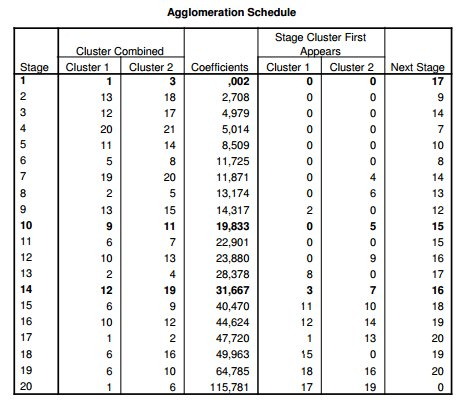
\includegraphics[scale=1.1]{images/AggloSc}\\
		%\caption{SPSS Agglomeration Schedule}
	\end{figure}
\end{center}
\begin{itemize}
	\item The procedure followed by cluster analysis at Stage 1 is to cluster the two cases that have the smallest
	squared Euclidean distance between them.
	\item  Then SPSS will recompute the distance measures between all
	single cases and clusters (there is only one cluster of two cases after the first step). 
	\item Next, the 2 cases (or
	clusters) with the smallest distance will be combined, yielding either 2 clusters of 2 cases (with 17 cases
	unclustered) or one cluster of 3 (with 18 cases unclustered). 
	\item  This process continues until all cases are clustered into a single group.
	For the sake of clarify, we will explain Stages 1, 10, and 14.
\end{itemize}




\subsubsection*{Stage 1}
\begin{itemize}
	\item At Stage 1, Case 1 is clustered with Case 3. The squared Euclidean distance between these two cases is
	0.002. 
	\item Neither variable has been previously clustered (the two zeros under Cluster 1 and Cluster 2), and the
	next stage (when the cluster containing Case 1 combines with another case) is Stage 17. 
	\item (\textit{Note that at Stage
	17, Case 2 joins the Case-1 cluster.})
\end{itemize}


\subsubsection*{Stage 10}
\begin{itemize}
	\item At Stage 10, Case 9 joins the Case-11 cluster (Case 11 was previously clustered with Case 14 back in Stage
	5, thus creating a cluster of 3 cases: Cases 9, 11, and 14). 
	\item The squared Euclidean distance between Case 9
	and Case-11 cluster is 19.833. 
	\item Case 9 has not been previously clustered (the zero under Cluster 1), and
	Case 11 was previously clustered at Stage 5. 
	\item The next stage (when the cluster containing Case 9 clusters) is
	Stage 15 (when it combines with the Case-6 cluster).
\end{itemize}


\subsubsection*{Stage 14}
\begin{itemize}
	\item At Stage 14, the clusters containing Cases 12 and 19 are joined, Case 12 has been previously clustered with
	Case 17, and Case 19 had been previously clustered with Cases 20 and 21, thus forming a cluster of 5 cases
	(Cases 12, 17, 19, 20, 21). 
	\item The squared Euclidean distance between the two joined clusters is 31.667. 
	\item Case
	12 was previously joined at Stage 3 with Case 17. Case 19 was previously joined at Stage 7 with the Case-
	20 cluster. 
	\item The next stage when the Case-12 cluster will combine with another case/cluster is Stage 16
	(when it joins with the Case-10 cluster).
\end{itemize}


\begin{figure}
	% Requires \usepackage{graphicx}
	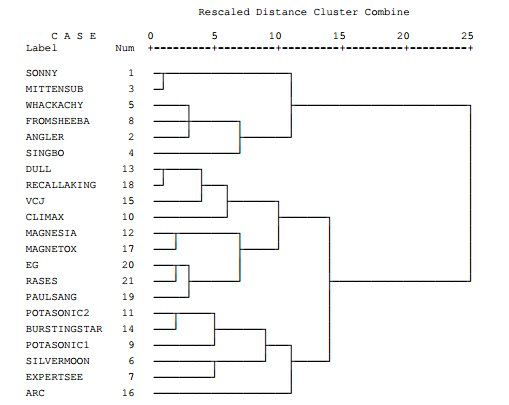
\includegraphics[scale=1.0]{images/Dendro}\\
	\caption{Corresponding Dendrogram}
\end{figure}

The branching-type nature of the Dendrogram allows you to trace backward or forward to any individual
case or cluster at any level. It, in addition, gives an idea of how great the distance was between cases or
groups that are clustered in a particular step, using a 0 to 25 scale along the top of the chart. While it is
difficult to interpret distance in the early clustering phases (the extreme left of the graph), as you move to
the right relative distance become more apparent. The bigger the distances before two clusters are joined,
the bigger the differences in these clusters. To find a membership of a particular cluster simply trace
backwards down the branches to the name.

%----------------------------------------------------- %
\newpage
\section{Non-Hierarchical Clustering}
\noindent \textbf{\textit{(Remark: This material provides a dove-tail with the next topic: K-means Clustering)}}\\ \smallskip
\begin{itemize}
\item This method of clustering is very different from the hierarchical clustering and Ward method, which are applied when there is no prior knowledge of how many clusters there may be or what they are characterized by.
\item  The k-means clustering approach is used when you already have hypotheses concerning the number of clusters in your cases or variables. For example, you may want to specify exactly three clusters that are to be as distinct as possible.
\item 
This is the type of research question that can be addressed by the k-means clustering algorithm. In general, the k-means method will produce the exact k different clusters demanded of greatest possible distinction. Very often, both the hierarchical and the k-means techniques are used successively.
\begin{itemize}
	\item[$\ast$] Ward's method is used to get some sense of the possible number of clusters and the way they merge as seen from the dendrogram.
\item[$\ast$] Then the clustering is rerun with only a chosen optimum number in which to place all
	the cases (i.e. k means clustering).
\end{itemize}
\item Non-hierarchical cluster analysis tends to be used when large data sets are involved. It is
sometimes preferred because it allows subjects to move from one cluster to another (this is
not possible in hierarchical cluster analysis where a subject, once assigned, cannot move to a
different cluster). 
\item Two disadvantages of non-hierarchical cluster analysis are: 
\begin{itemize}
	\item[1]it is often
	diffcult to know how many clusters you are likely to have and therefore the analysis may have
	to be repeated several times 
	\item[2] it can be very sensitive to the choice of initial cluster centres. Again, it may be worth trying di?erent ones to see what impact this has.
\end{itemize}
\end{itemize}
\subsection{Optimal Number of Clusters}
One of the biggest problems with cluster analysis is identifying the optimum number of
clusters. As the joining process continues, increasingly dissimilar clusters must be joined. i.e. the classification becomes increasingly artificial. Deciding upon the optimum number
of clusters is largely subjective, although looking at a dendrogram would help.

% http://www.uk.sagepub.com/burns/data.htm
% Data Set 23 A

% DASL
% http://lib.stat.cmu.edu/cgi-bin/dasl.cgi?query=Cluster+analysis&submit=Search%21&metaname=methods&sort=swishrank

\end{document}

\newpage
\section{Errata}
\subsection{Unknown Example}
\begin{itemize}
	\item 
	The hierarchical clustering procedure attempts to identify relatively homogeneous groups of cases (or variables) based on selected
	characteristics. For example: cluster television shows into homogeneous groups based on viewer
	characteristics. In hierarchical clustering, an algorithm is used that starts with each case (or variable) in a
	separate cluster and combines clusters until only one is left.
	\item 
	
	
	To cluster cases you need to identify variables you wish to be considered in creating clusters for the cases.
	The variables to be used for cluster formation are here: picture quality (5 measures), reception quality (3
	measures), audio quality (3 measures), ease of programming (1 measure), number of events (1 measure),
	number of days for future programming (1 measure), remote control (3 measures), and extras (3 measures).
	Pass these in the Variable(s) box.
	\item 
	Cluster Method: Choose the procedure for combining clusters. The default procedure is called the
	between-group linkage. SPSS computes the smallest average distance between all group pairs and
	combines the two groups that are closest. 
	\item The procedure begins with as many clusters as there are cases
	(here: 21). At step one, the two cases with the smallest distance between them are clustered. Then SPSS
	computes distances once more and combines the two that are next closest. 
	\item After the second step you will
	have either 18 individual cases and one cluster of 3 cases, or 17 individual cases and two clusters of two
	cases each. The process continues until all cases are grouped into one large cluster.
	Measure: Indicate what method is used for distance measuring, the default is Squared Euclidean distance. 
\end{itemize}